%\documentstyle[epsf,twocolumn]{jarticle}       %LaTeX2.09仕様
%\documentclass[twocolumn]{jarticle}     %pLaTeX2e仕様
\documentclass{jarticle}     %pLaTeX2e仕様

\setlength{\topmargin}{-45pt}
%\setlength{\oddsidemargin}{0cm} 
\setlength{\oddsidemargin}{-7.5mm}
%\setlength{\evensidemargin}{0cm} 
\setlength{\textheight}{24.1cm}
%setlength{\textheight}{25cm} 
\setlength{\textwidth}{17.4cm}
%\setlength{\textwidth}{172mm} 
\setlength{\columnsep}{11mm}

\kanjiskip=.07zw plus.5pt minus.5pt

\usepackage{graphicx}
\usepackage[dvipdfmx]{color}
\usepackage{subcaption}
\usepackage{enumerate}
\usepackage{comment}
\usepackage{url}
\usepackage{multirow}
\usepackage{diagbox}
\usepackage{bm}
\usepackage{amssymb}
\usepackage{amsfonts}
\usepackage{booktabs}



\begin{document}
  \noindent
  \onecolumn
  \hspace{1em}

  \today
  \hfill
  \ \  学籍番号1201201100 西村昭賢 

  \vspace{2mm}
  \hrule
  \begin{center}
  {\Large \bf 情報工学英語演習 「{\rm AttentionIsAllYouNeed}」の和訳}
  \end{center}
  \hrule
  \vspace{3mm}

\section*{Abstruct}
今までの主要なsequence transduction modelは,エンコーダーとデコーダーを含む
複雑なRNNやCNNに基づいていた.最も良いパフォーマンスであったモデルも,エンコーダーとデコーダーをアテンションの仕組みを用いて接続しているモデルであった.\par
私達は,RNNやCNNを用いず,アテンションのみからなるTransformerと呼ばれる新しい簡潔なモデルを提案する.2回の翻訳実験の結果,Transformerは今までのモデルより優れており,更には,より並列化が可能で学習の時間も少ないことが分かった.
TransformerはWMT2014英独翻訳タスクにおいて,「プロの翻訳者の訳と近ければ近いほどその機械翻訳の精度は高い」という考え方に基づく機械翻訳の評価方法であるBLEUスコアで28.4BLEUを記録した.これは,複数のモデルを融合させて1つの学習モデルを生成するアンサンブル学習を含めたこれまでの最高記録を2BLEU上回る結果であった.また、WMT2014英仏翻訳タスクにおいては、8個のGPUを用いた3.5日の学習というこれまでの最先端のモデルの学習よりも遥かに少ないコストで,41.0BLEUという単一モデルの最高記録を打ち立てた.

%TODO sequence transduction modelの自然な訳、時系列分析モデル?


\section{Introduction}
RNN,特にRNNにおいて文章の長期的な依存関係を学習できるようにしたLSTMやgated RNNは,言語モデルや機械翻訳などのSequence 問題への最適な手法として確固たる地位を築いていた.
それ以来,Recurrent言語モデルとエンコーダー-デコーダー構造の限界を押し上げる数々の努力がなされてきた.
\par
リカレントモデルでは,通常,入力と出力の時系列データの時間的な位置に沿って計算を行う.
よって計算は逐次的に行われ,時刻$t$における隠れ状態$h_\mathrm{t}$は,時刻$t-1$の隠れ状態の$h_\mathrm{t-1}$と時刻$t$における入力から導かれる.
このように本質的に逐次的な性質を孕んでいるため,学習の並列処理が困難である.そのため,メモリの制約上,長い時系列データなどの学習には致命的であった.
直近の研究ではfactorization tricksやconditional computationといった方法で計算効率がかなり改善され,後者ではモデルの性能まで向上させることができたが,逐次的な計算の問題は残ったままだった.\par
Attentionは入力と出力の時系列データにおける距離を気にせず依存関係をモデル化することができ,様々なタスクにおいて有効なsequence modelとtransduction modelの必要不可欠な部分となっている.しかし,一部の場合にはAttentionはRNNと合わせて用いられる.\par
本研究で私達が提案するTransformerは,RNNを用いず,Attentionのみで入力と出力の完全な依存関係を取り出すモデルのアーキテクチャである.
Transformerは学習の並列処理が可能であり,8個のP100 GPUで12時間という小規模な学習後に,最高の機械翻訳性能に達することができた.


\section{BackGround}
逐次的な計算を減らすという目標は,Extended Neural GPU,ByteNet,ConvS2Sといったモデルの基礎にもなっている.これらはどれもCNNを基本構成要素として,入力と出力のすべての位置で隠れ状態の値を計算する.またこれらのモデルにおいて,任意の入力の位置と出力の位置の信号を関連付けるために必要な計算時間は,ConvS2Sdでは線形的,ByteNetでは指数的となる.
そのため離れた位置の依存関係を学習することはより困難になる.
Transformerでは,この計算時間を定数時間に減らすことができる.Attentionで重み付けした位置を平均化することで有効な解像度が下がってしまうが,3.2説で述べるMulti-Head Attentionにより相殺できる.\par

intra-attentionとも呼ばれるSelf-Attentionは,単一の文章の異なる位置を関連付けるAttentionである.Self-Attentionは文章読解,要約,テキスト含意,独立した文の表現の学習などのタスクで用いられ成功している.\par

End-to-End memory NetworksはRNNの代わりに再帰的なAttentionを元にしており,単純な言語の質疑応答,言語モデリングといったタスクにおいて優れた結果を示している.\par

しかし私達が知る限り,TransformerはRNNやCNNを用いずに入出力の表現を計算するために,Self-Attentionのみに依存した最初のtransduction modelである.次節以降では,Transformer,self-attentionについて説明しこれまでのモデルと比較した利点を議論する.




\section{Model Architecture}
最も優位性のあるsequence transduction modelsはエンコーダー-デコーダー構造を有している.エンコーダーは配列で表現される入力($x_\mathrm{1}$,...,$x_\mathrm{n}$)を配列\bm{$z$}=($z_\mathrm{1}$,...,$z_\mathrm{n}$)に変換する.
デコーダーは\bm{$z$}から出力として配列($y_\mathrm{1}$,...,$y_\mathrm{n}$)を1要素ずつ出力する.
このステップで,モデルが生成する要素はこれまでに生成した要素のみに依存する自己回帰モデルであり,直前に生成された要素を新しく入力として次の要素を生成する.\par
Transformerは図1の左半分と右半分に示すように,全体としてはエンコーダー-デコーダー構造を踏襲しつつ,self-attention層とpoint-wise全結合層を積み重ねた層を使用している.

\begin{figure}[ht]
  \centering
  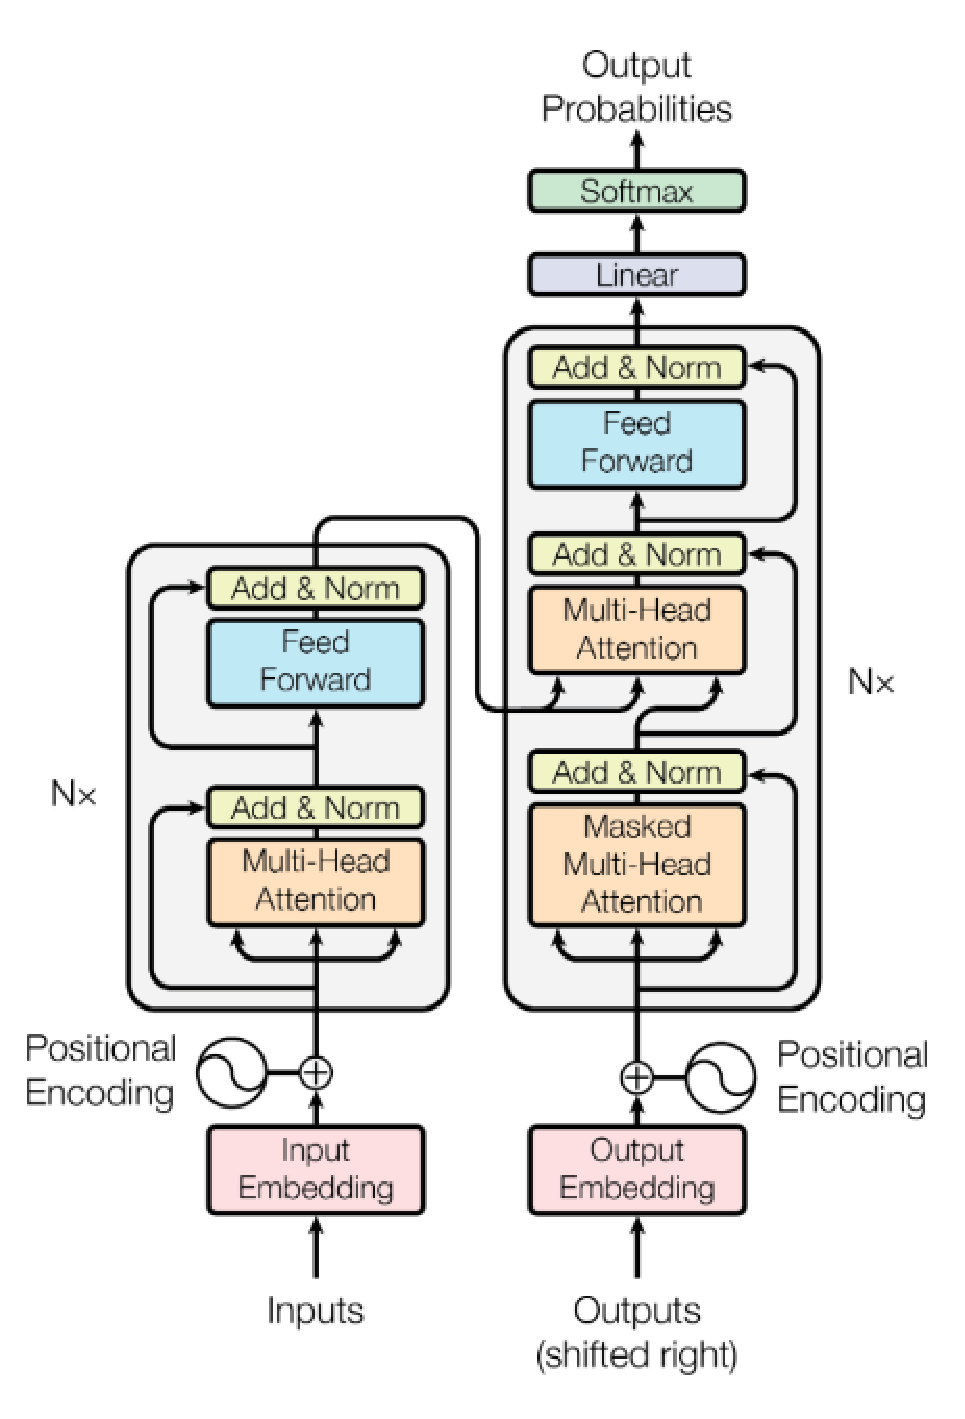
\includegraphics[width=100mm]{assets/Figure1.eps}
  \caption{Transformerのモデルアーキテクチャ.}
  \label{Figure1}
\end{figure}


\subsection{Encoder and Decoder Stacks}
エンコーダー: 6層からなり,各層は全く同じ構造である.それぞれの層は2つの下位層を持ち,下位層の後には残差接続や標準化が行われている.
よって,下位層自身の出力をSublayer($x$)として,下位層全体としての出力はLayerNorm($x$+Sublayer($x$))となる.残差接続を容易にするために,すべての下位層,embedding layersも出力の次元を$d_\mathrm{model}$=512としている.\par
\par
デコーダー: デコーダーも同一の6層からなる.エンコーダーの2つの下位層に加えて,エンコーダーの出力を入力として受ける3つ目の下位層を加えている.エンコーダーと同じく,下位層の後には残差接続や標準化が行われている.ただ,self-attention下位層は改良しており,後続の要素が影響しないようにしている.このマスキングと,出力が1要素ごと補われることを組み合わせることで,マスキングにより地点$i$での予測が地点$i$未満での既知の出力のみに依存することが保証される.

\subsection{Attention}
アテンションの仕組みは,クエリとキーとキー値のセットを出力へマッピングし,クエリやキー,キー値,出力はすべてベクトルである.出力はキー値の重み付き和として計算され,それぞれのキー値へ割り当てられる重みはクエリとクエリに対応するキーからの変換関数で計算される.

\subsubsection{Scaled Dot-Product Attention}
私が独自に考案したアテンションを"Scaled Dot-Product Attention"と呼ぶ.図2にScaled Dot-Product Attentionのアーキテクチャを示す.\par

\begin{figure}[ht]
  \centering
  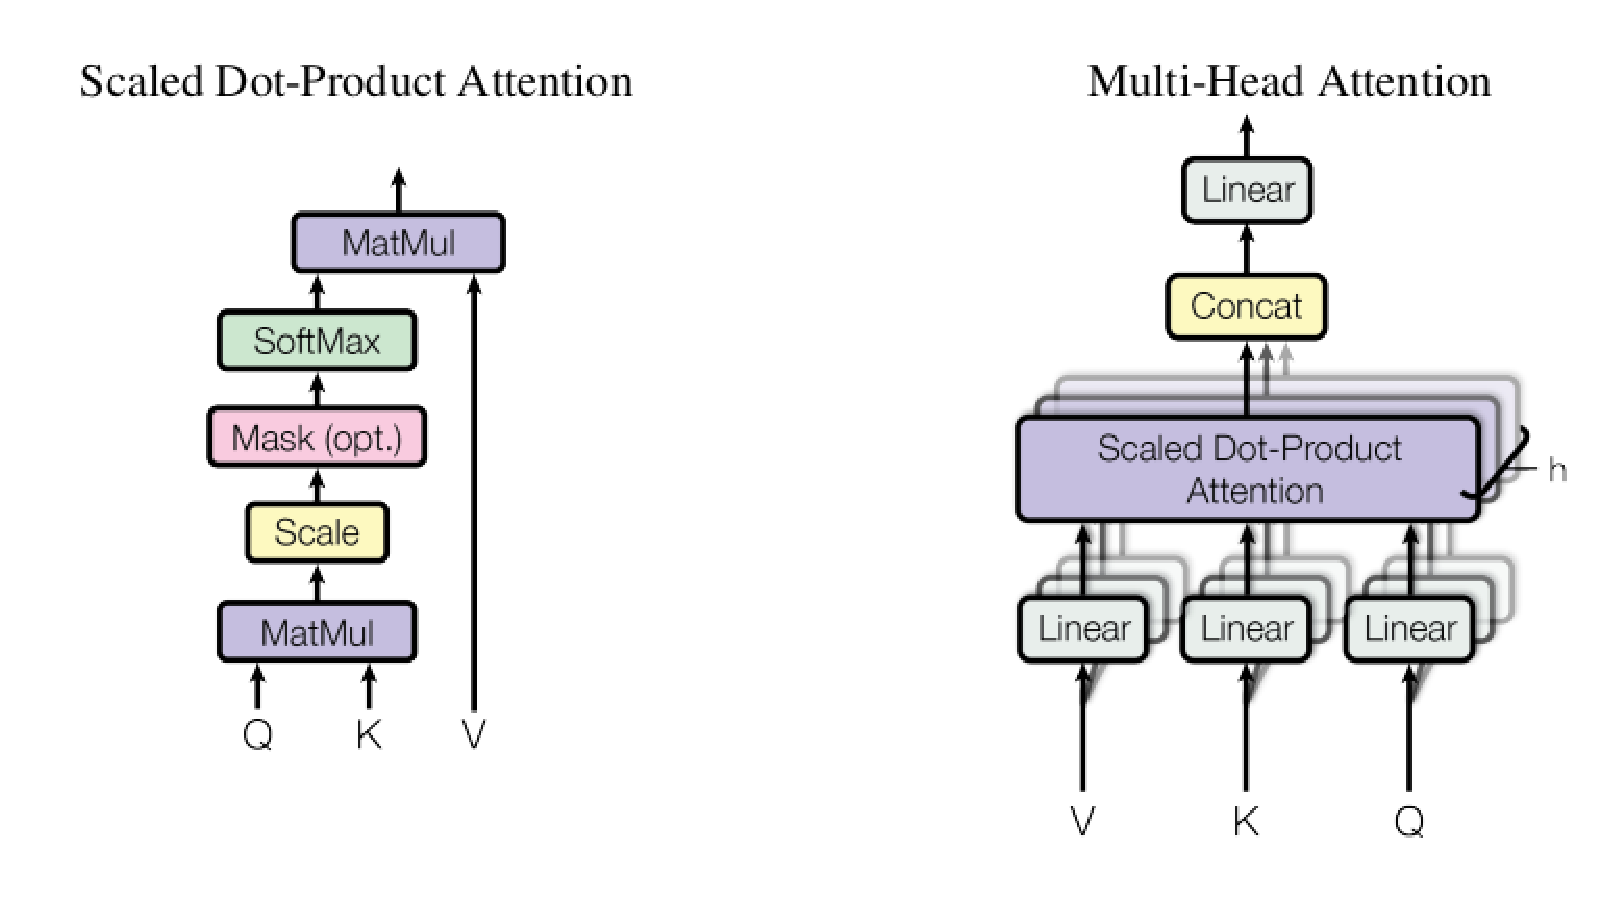
\includegraphics[width=100mm]{assets/Figure2.eps}

  \caption{(左)Scaled Dot-Product Attention. (右)複数のアテンション層が並列に構成されているMulti-Head Attention.}
  \label{Figure2}
\end{figure}


入力はクエリと次元$d_\mathrm{k}$のキー,次元$d_\mathrm{v}$のキー値からなる.クエリとキーの内積を計算し,それを$\sqrt{d_\mathrm{k}}$で割り,キー値の重みを得るためにsoftmax関数を適用する.
実際にはクエリを行列$Q$としてまとめて同時に計算している.キーやキー値も同様に行列$K$,$V$にまとめて計算している.行列による出力は(1)式のように表せる.

\begin{equation}
  \mathrm{Attention}(Q,K,V) = \mathrm{softmax}(\frac{QK^T}{\sqrt{d_\mathrm{k}}})V
\end{equation}

\par

最も一般的に利用されるAttentionとしてはadditive attentionとdot-product attentionの2つがある.Dot-product attentionは,Scaled Dot-Product Attentionから$\sqrt{d_\mathrm{k}}$で割る処理を除いたものである.Additive attentionは一つの隠れ層を持つfeed-forward networkを用いて変換関数を計算している.2つのAttentionは理論的には似ているが,高度に最適化された行列積のコードを内包しているためdot-product attentionのほうが計算が遥かに早く,メモリ効率も良い.\par
$d_\mathrm{k}$が小さい値である時はこの2つのAttentionは同様に作用するが,$d_\mathrm{k}$が大きい値である時には,Additive attentionは標準化をしないdot-product attentionより性能が良くなる.私達は,$d_\mathrm{k}$が大きい値である時に,内積の値が急激に増加し,softmax関数の勾配消失が起こると考え,それを防ぐために内積を$\frac{1}{\sqrt{d_\mathrm{k}}}$で標準化している.

\subsubsection{Multi-Head Attention}
次元$d_\mathrm{model}$におけるキーとキー値とクエリを用いた単一のattention関数を使用する代わりに,クエリとキーとキー値に$h$回線形射影を行い,次元を$d_\mathrm{k}$,$d_\mathrm{k}$,$d_\mathrm{v}$にそれぞれ削減したほうが都合が良いと判明した.
射影したクエリ,キー,キー値それぞれに対して,Attention関数を並列に実行し,次元$d_\mathrm{v}$の出力を得る.それらをConcat層で連結し,もう一度線形射影して最終的な出力を得る.図2にこの一連の過程を示す.
\par
Multi-Head Attentionにより,異なる要素の異なる部分ベクトル空間を見ることができる.single attention headでは,平均化によりこのようなことはできない.
\par
\begin{eqnarray*}
  \mathrm{MultiHead}(Q,K,V)&  = & \mathrm{Concat}(head_\mathrm{1},...,head_\mathrm{h})W^O   \\
  ここで, head_\mathrm{i} & = & \mathrm{Attention}(QW_\mathrm{i}^Q,KW_\mathrm{i}^K,VW_\mathrm{i}^V)
\end{eqnarray*}

射影関数のパラメータの行列は,
$W_\mathrm{i}^Q \in \mathbb{R} ^ {{d_\mathrm{model}} \times {d_\mathrm{k}}}$,\par
$W_\mathrm{i}^K \in \mathbb{R} ^ {{d_\mathrm{model}} \times {d_\mathrm{k}}}$,
$W_\mathrm{i}^V \in \mathbb{R} ^ {{d_\mathrm{model}} \times {d_\mathrm{v}}}$と\par
$W_\mathrm{i}^O \in \mathbb{R} ^ {{hd_\mathrm{v}} \times {d_\mathrm{model}}}$である.

本研究では,$h=8$の並列のattention層を用いて,次元を
$d_\mathrm{k} = d_\mathrm{v} = d_\mathrm{model}/h = 64$とした.
次元の削減により,総計算コストを,次元の削減を行わなかった場合の単一のattentionと同等まで削減することができた.

\subsubsection{Applications of Attention in our Model}
Transformerでは,multi-head attentionを以下の3つの方法で採用している.
\begin{itemize}
  \item "encoder-decoder attention"層では,クエリは直前のデコーダー層から生まれ,キーとキー値はエンコーダーの出力から生まれる.デコーダー内のすべての要素が入力文のすべての要素を見ることができる.これは,sequence to sequenceモデルの典型的なencoder-decoder attentionを模倣している.
  \item エンコーダはself-attention層を含んでいる.self-attention層では,キー,キー値,クエリの全てが,エンコーダー内の一つ前の層の出力から生まれている.エンコーダー内のそれぞれの要素は,エンコーダーの一つ前の層の,その要素までの全ての要素を見ることができる.
  \item 同様に,デコーダー内のself-attention層も,デコーダーの全層の要素を参照することができるが,自動回帰的な特性を保持するために,左向きへの情報の流出を防がなければならない.すなわち,翻訳済の単語に影響が出ないようにしなければ行けない.私達はscaled dot-product attentionの中で,不当な接続に相当する部分を-$\infty$にマスキングして,softmax層の入力として与えることで,これを実現している.図2にこの過程を示している.
\end{itemize}

\subsection{Position-wise Feed-Forward Networks}
Attentionの下位層に加えて,エンコーダーとデコーダーのそれぞれの層には,完全に連結したfeed-forward networkが含まれている.feed-forward networkは,2つの線形変換の間にReLU関数を適用した形となっている.

\begin{equation}
  \mathrm{FFN}(x) = \mathrm{max}(0,xW_\mathrm{1}+b_\mathrm{1})W_\mathrm{2} + b_\mathrm{2}
\end{equation}

線形変換は異なる要素に対しても同じ値を掛けるのに対して,層を変えることに異なるパラメータを用いる.言い換えると,カーネルサイズが1の2つの畳み込みとして捉えることができる.
入出力の次元は$d_\mathrm{model} = 512$とし,feed-forward network内では次元は$d_\mathrm{ff} = 2048$としている.

\subsection{Embeddings and Softmax}
他のsequence transduction modelと同様に,学習済みのembeddingを用いて入力と出力のトークンを次元$d_\mathrm{model}$のベクトルに変換する.また,一般的な学習済みの線形変換とsoftmax関数を用いてデコーダーの出力を予測済みのnext-tokenの予測確率に変換している.私達のモデルは,2つのembedding層とsoftmax層の前の線形変換で同じ重み行列を使用している.また,embedding層では$\sqrt{d_\mathrm{model}}$を掛けている.

\subsection{Positional Encoding}
私達のモデルはRNNやCNNを含んでいないため,モデルが要素の順番を利用するために,絶対的であれ,相対的であれ何らかの要素の順番の情報を定義する必要があった.結果として,"positional encoder"を入力のembedding層に付け加え,エンコーダーとデコーダーの最下層に入れることとした.embedding層との加算を行うために,positional encodingの次元はembeddingと同じ$d_\mathrm{model}$とした.\par
本研究では,positional encodingとして別々の周波数を持つsin関数,cos関数を用いた.

\begin{eqnarray*}
  PE_{(pos,2i)} &= &sin(pos/10000^{2i/d_\mathrm{model}}) \\
  PE_{(pos,2i+1)} &= &cos(pos/10000^{2i/d_\mathrm{model}})
\end{eqnarray*}

ここで,$pos$は要素の位置,$i$は次元である.つまり,position encodingのそれぞれの次元は正弦波に該当する.波長は$2\pi$から$10000・2\pi$まで段階的に増加していく.この関数を採用した理由は,モデルが相対的な位置から参照できるように簡単に学習できると仮設を立てたためである.なぜなら,任意の定数オフセット$k$において,$PE_{pos+k}$は$PE_{pos}$の線形関数として表すことができるからだ.\par
別の論文の学習済みのpositional embeddingを用いた実験を行ったところ,本論文と別論文の結果はほぼ等しくなった.そこで,学習時よりもより長いデータに対しても対応できると判断し正弦波verを採用した.


\section{Why Self-Attention}

本章では,self-attention層における様々な側面を,RNNやCNNと比較する.RNNやCNNは可変長の配列
($x_\mathrm{1}$,...,$x_\mathrm{n}$)を,同じ長さの配列($z_\mathrm{1}$,...,$z_\mathrm{n}$)に変換し,エンコーダーやデコーダーなどの典型的なsequence transductionの隠れ層に用いられる.私達がself-attentionを使う理由としては,3つの大きな不足を感じる物事があったからである.
\par
1つ目は層ごとの計算の複雑さである.2つ目は本来並列化が可能な計算量である.これは必要最低限の配列計算量から算出できる.
\par
3つ目がモデルのネットワークで遠い位置関係の要素の依存関係を認識できる経路の長さである.
遠い位置関係の要素の依存関係を学習することは,多くのsequence transductionタスクにおいて重要な課題である.そのような依存関係を学習するための1つの重要な要因は順方向か逆方向かの信号がネットワークを通る経路の長さである.入力と出力の位置関係の間の経路が短ければ短いほど,より長い位置関係での依存関係の学習が容易になる.従って,私達は異なる種類の層からなるネットワークにおいての入力と出力の位置間の最大の経路長を比較した.表1にその結果を示す.

\begin{table}[hbtp]
  \caption{異なる種類の層における層ごとの計算の複雑さ,配列計算の計算量,最大経路長.$n$は配列の長さ,$d$は表現の次元,$k$はCNNのカーネルのサイズ,$r$は制限付きSeld-Attentionの近傍サイズ.}
  \label{table:path length}
  \small
  \centering
  \scalebox{1.2}[1.2]{
    \begin{tabular}{lccc}
      \hline
      Layer Type  & Complexity per Layer  &  Sequential Operations & Maximum Path Length \\
      \hline 
      Self-Attention  & $O(n^2・d)$  & $O(1)$ & $O(1)$ \\
      Recurrent  & $O(n・d^2)$   & $O(n)$ & $O(n)$ \\
      Convolutional  & $O(k・n・d^2)$  & $O(1)$ & $O(log_k(n))$ \\
      Self-Attentional(restricted)  &  $O(r・n・d)$  &  $O(1)$ & $O(n/r)$ \\
      \hline
    \end{tabular}
  }
  
\end{table}

表1で示した通り,配列計算にRNNが$O(n)$時間かかるのに対して,Self-Attentionは$O(1)$時間,すなわち定数時間で行うことができる.計算の複雑さという観点では,一般的に機械翻訳での文の表現では$n<d$であることから,Self-AttentionはRNNより優れていると言える.
非常に長い文章に関するタスクに関して計算のパフォーマンスを向上させるためには,それぞれの予測に対応する入力文のサイズ$r$の範囲しか考えないという制限をSelf-Attentionに課す方法がある.しかし,この方法では,最大経路長が$O(n/r)$となってしまう問題がある.これは将来の研究の課題である.
\par
カーネルのサイズ$k$が,$k<n$となるような1層のCNNは,入力と出力の全てのペアを関連付けることはできない.そうするためには,連続したカーネルの場合は$O(n/k)$の積み重なった畳み込み層が必要,膨張畳込みの場合でも$O(log_k(n))$の層が必要となる.このため,最大経路長が増えてしまう問題が生じる.CNN層は,カーネルのサイズ$k$により,一般的にRNN層よりも計算が複雑になる.しかし,Separable convolutionsは計算の複雑さを$O(k・n・d + n・d^2)$まで減らしている.$k=n$の場合,Separable convolutionsは本研究で採用しているself-attention層とpoint-wise feed-forward network層の組み合わせと計算の複雑さは等しくなる.
\par
良い面として,self-attentionはより解釈しやすいモデルを得ることができる.モデルのattention分布について,付録で例を示して議論する.Attentionはそれぞれのタスクをきちんと学習するだけでなく,文の構文規則や意味構造になぞらえた振る舞いをしているようだ.

\section{Training}
本章では,私達のモデルの学習計画について記載する.

\subsection{Training Data and Batching}
英独翻訳に関して,450万もの文からなるstanderd WMT 2014 English-Germanデータセットを用いて学習を行った.文はbyte-pair encodingでエンコードされており,約37,000個のトークンの語彙が共有されている.英仏翻訳では,3600万もの文からなる大規模なWMT 2014 English-Frenchデータセットを用いた.トークンを32,000個の語彙に分割して使用した.文のペアはおおよその文の長さでバッチ処理を行った.それぞれの学習用バッチは文章対がまとまっており,おおよそ25,000個のsource token,target tokenが含まれる.

\subsection{Hardware and Schedule}
モデルの学習は,8個のNVIDIA P100 GPUを搭載した1つの計算機で行った.
本論文で述べたハイパーパラメータを使ったベースモデルでは,訓練の1ステップあたり0.4秒かかった.ベースモデルは100000ステップの合計で12時間学習を行った.大きいモデルでは1ステップあたり1.0秒かかり,300000ステップ,計3.5日かかった.

\subsection{Optimizer}
optimizerとしてAdamを用いた.パラメータは$\beta_\mathrm{1} = 0.9$,$\beta_\mathrm{2} = 0.98$, $\epsilon = 10^{-9}$とした.学習率は学習を行うに従って以下の式に応じて変更した.

\begin{equation}
  lrate = d_\mathrm{model}^{-0.5}・\mathrm{min}(step\_num^{-0.5},step\_num・warmup\_steps^{-1.5})
\end{equation}

学習の際,学習率は$warmup\_step$まで線形的に増えていくが,それ以降のステップでは,ステップ数の平方根の逆数に比例して減少していく.

\subsection{Regularization}
実験の際,3つの正則化を採用した.

\textbf{Residual Dropout}
それぞれの下位層の出力が残差接続される前にDropout処理を行った.それに加えて,エンコーダーとデコーダー両方のembeddingsとpositional encodingの和にもDropout処理を行った.ベースモデルでは,$P_{drop} = 0.1$とした.

\textbf{Label Smoothing}
学習中,$\epsilon_{ls} = 0.1$としてLabel Smoothingを行った.モデルが曖昧さを学ぶことで,翻訳の正確さの指標であるperplexityは減るものの,BLEUスコアは向上する.

\section{Results}


\subsection{Machine Translation}
WMT2014英独翻訳において,表2に示すように,bigモデルがアンサンブルを含む既知のモデルに2.0BLEU以上の差をつけて28.4BLEUという最高記録を打ち立てた.表3の下部にこのモデルの構成要素を示す.学習は8個のP100 GPUで3.5日間かかった.baseモデルは,既存のモデルやアンサンブルに比べて良いBLEUスコアを残している上に,既存のモデルに比べて数分の1の計算コストで学習を行っている.
\par
WMT2014英仏翻訳タスクに関して,bigモデルでは41.0BLEUスコアを記録している.既存の単一のモデルの全てより良いスコアであり,既存の最良のモデルに比べ1/4以下の学習コストで学習を行っている.bigモデルは英仏翻訳タスクに関しては,Dropout rate $P_{drop}$を0.3の代わりに0.1と設定している.
\par

baseモデルでは,10分感覚で保存されるチェックポイントの最後の5回分を平均化したモデルとした.bigモデルは最後の20回分を平均化した.また,beam sizeを4,Length Penaltyの$\alpha=0.6$としてbeam searchを使用している.これらのハイパーパラメータは開発セットの実験後に決定した.
推論時の出力の最大長は入力の長さ+50までとし,可能なら早めに打ち切るようにした.
\par
表2に,本研究のモデルと参考文献のモデルとの翻訳の質と計算コストを示す.

\begin{table}[h]
  \caption{Transformerは,英独翻訳,英仏翻訳の2014年最新のタスクで以前の最先端のモデルに比べ,僅かな計算コストで良いBLEUスコアを残した.}
  \label{table:Transformer}
  \centering
   \begin{tabular}{lcccc}
    \toprule             % --- booktabs: 上の罫線 ---
    model & \multicolumn{2}{c}{BLEU} & \multicolumn{2}{l}{Training Cost(FLOPs)}\\
    \cmidrule(lr){2-3}
    \cmidrule(lr){4-5}
     & EN-DE & EN-FR & EN-DE & EN-FR \\
    \midrule             % --- booktabs: 中間の罫線 ---
    ByteNet & 23.75 & & & \\
    Deep-Att + PosUnk & & 39.2 & & 1.0・$10^{20}$ \\
    GNMT + RL & 24.6 & 39.92 & 2.3・$10^{19}$ & 1.4・$10^{20}$ \\
    ConvS2S & 25.16 & 40.46 & 9.6・$10^{18}$ & 1.4・$10^{20}$ \\
    MoE & 26.03 & 40.56 & 2.0・$10^{19}$ & 1.2・$10^{20}$ \\
    \hline
    Deep-Att + PosUnk Ensemble & & 40.4 & & 8.0・$10^{20}$ \\
    GNMT + RL Ensemble & 26.30 & 41.16 & 7.7・$10^{20}$ & 1.2・$10^{20}$ \\
    ConvS2S Ensemble & 26.36 & \textbf{41.29} & 7.7・$10^{19}$ & 1.2・$10^{21}$ \\
    \hline
    Transformer(base model) & 27.3 & 38.1 & \multicolumn{2}{c}{\bf{3.3・$\mathbf{10^{18}}$}} \\
    Transformer(big) & \textbf{28.4} & \textbf{41.0} &  \multicolumn{2}{c}{2.3・$10^{19}$}\\ 
    \bottomrule          % --- booktabs: 底の罫線 ---
   \end{tabular}
 \end{table}

Training Costとして,コンピュータが1秒間に処理可能な浮動小数点演算の回数を表したFLOPsを用いており,学習時間,GPUの使用数,それぞれのGPUにおける処理可能な単精度浮動小数点の推定値をかけ合わせて計算した.

\subsection{Model Variations}
Transformerの各構成要素を評価するために,baseモデルを様々に変化させ,Newest2013の開発セットにおける英独翻訳タスクでの性能を評価した.前節で述べたビームサーチを用いたが,チェックポイントの平均化は行わなかった.表3に結果を示す.


% TODO 表3作る

表3の(A)行では,3.2.2節で述べた通り計算量を一定にしたまま,Multi-Head Attentionのheadsの数$h$,キーやキー値の次元$d_\mathrm{k}$,$d_\mathrm{v}$を変化させた結果を示している.$h=1$の時は,最適なパラメータ設定のときに比べ,0.9ほどBLEUスコアが低くなっており,$h=32$など多すぎる場合もスコアが低くなっている.\par
(B)行では,Attentionのキーの次元$d_\mathrm{k}$の影響を観察した.結果として,優劣をつけるのは難しく,Scaled Dot-Product Attentionより良い変換関数があるかもしれない.(C),(D)行では,エンコーダー,デコーダーの層の数$N$,モデルの入出力の次元$d_\mathrm{model}$,Feed-Forward Networks内の次元$d_\mathrm{ff}$,DropoutやLabelSmoothingのパラメータ$P_{drop}$,$\epsilon_{ls} = 0.1$を変化させて実験を行った結果を示している.想定通り,パラメータを増やしモデルの規模を大きくするほどよい結果が得られ,またDropout処理は過学習を避けるために有効であった.行(E)では,本研究の正弦波を用いたpositional encodingを他の研究のpositional encodingと置き換えた結果を示しており,大きな違いは見られなかった.

\section{Conclusion}


%index.bibはtexファイルと同階層に置く
%ちゃんと\citeしないと表示されない(1敗)
\bibliography{index.bib}
\bibliographystyle{junsrt}

\end{document}